% document formatting
\documentclass[10pt]{article}
\usepackage[utf8]{inputenc}
\usepackage[left=1in,right=1in,top=1in,bottom=1in]{geometry}
\usepackage[T1]{fontenc}
\usepackage{xcolor}

% math symbols, etc.
\usepackage{amsmath, amsfonts, amssymb, amsthm}

% lists
\usepackage{enumerate}

% images
\usepackage{graphicx} % for images

% code blocks
\usepackage{minted, listings} 

% verbatim greek
\usepackage{alphabeta}

\graphicspath{{./assets/images/Week 2}}

\newcommand{\solution}{\textbf{Solution:}} 
\newcommand{\example}{\textbf{Example: }}
\newcommand{\water}{\text{H$_2$O}}
\newcommand{\hydroxide}{\text{OH$^-$}}
\newcommand{\hydronium}{\text{H$_3$O$^+$}}
\newcommand{\proton}{\text{H$^+$}}
\newcommand{\pc}{$^+$}
\newcommand{\nc}{$^-$}
\newcommand{\ka}{\text{$K_\text{a}$}}

\title{CHEM 153A Week 2}

\author{Aidan Jan}
\date{\today}

\begin{document}
\maketitle

\section*{Ionization Constants}
\begin{itemize}
    \item The tendency for any acid (HA) to lose a proton and form its conjugate base (A\nc) is defined by the equilibrium constant (K$_{\text{eq}}$) for the reversible reaction
    \begin{center}
        HA $\rightleftharpoons$ H\pc + A\nc
    \end{center}
    for which 
    \[K_{eq} = \frac{[\text{H}^+][\text{A}^-]}{[\text{HA}]} = K_a\]
\end{itemize}
\subsection*{Acid Strength Comparison: \ka ~and p\ka ~Values of Common Acids}
\begin{center}
    \begin{tabular}{|c|c|c|c|}
        \hline
        No. & \textbf{Acid} & $K_a$ & p$K_a$ \\ \hline
        1 & Hydroiodic acid (HI) & $3.16\times 10^9$ & -9.5 \\ \hline
        2 & Hydrobromic acid (HBr) & $1.0\times 10^9$ & -9 \\ \hline
        3 & Hydrochloric acid (HCl) & $1.0\times 10^6$ & -6 \\ \hline
        4 & Sulfuric acid (H$_2$SO$_4$) & $1.0\times 10^3$ & -3 \\ \hline
        5 & Hydronium ion (\hydronium) & $55$ & -1.74 \\ \hline
        6 & Nitric acid (HNO$_3$) & $28.2$ & -1.45 \\ \hline
        7 & Trifluoroacetic acid (CF$_3$COOH) & $5.62\times 10^{-1}$ & 0.25 \\ \hline
        8 & Oxalic acid (HOOC-COOH) & $5.37\times 10^{-2}$ & 1.27 \\ \hline
        9 & Acetic acid (CH$_3$COOH) & $1.75\times 10^{-5}$ & 4.76 \\ \hline
        \end{tabular}
\end{center}

\subsection*{p\ka}
\begin{itemize}
    \item p\ka = analogous to pH and defined by the equation
    \[p\ka = \log \frac{1}{\ka} = -\log \ka\]
    \item the stronger the tendency to dissociate a proton, the \underline{\textbf{stronger the acid} and \textbf{the lower its p\ka}}
    \item p\ka can be determined experimentally
\end{itemize}
\subsection*{Titration Curves Reveal the p\ka of Weak Acids}
\begin{itemize}
    \item titration curve = a plot of pH against the amount of OH equivalents added
\end{itemize}
\begin{center}
    \includegraphics*[scale=0.8]{L1_1.png}
\end{center}
\subsubsection*{Comparison of the Titration Curves of Three Weak Acids}
\begin{itemize}
    \item a \textbf{weak acid} and its anion - a conjugate acid-base pair - can act as a \textbf{buffer}
    \item Titration curves for acetic acid, dihydrogen phosphate, and ammonium are shown below
    \item \textbf{Conjugate acid-base pairs are effective buffers between approximately 10\% and 90\% neutralization of the proton donor species}
\end{itemize}
\begin{center}
    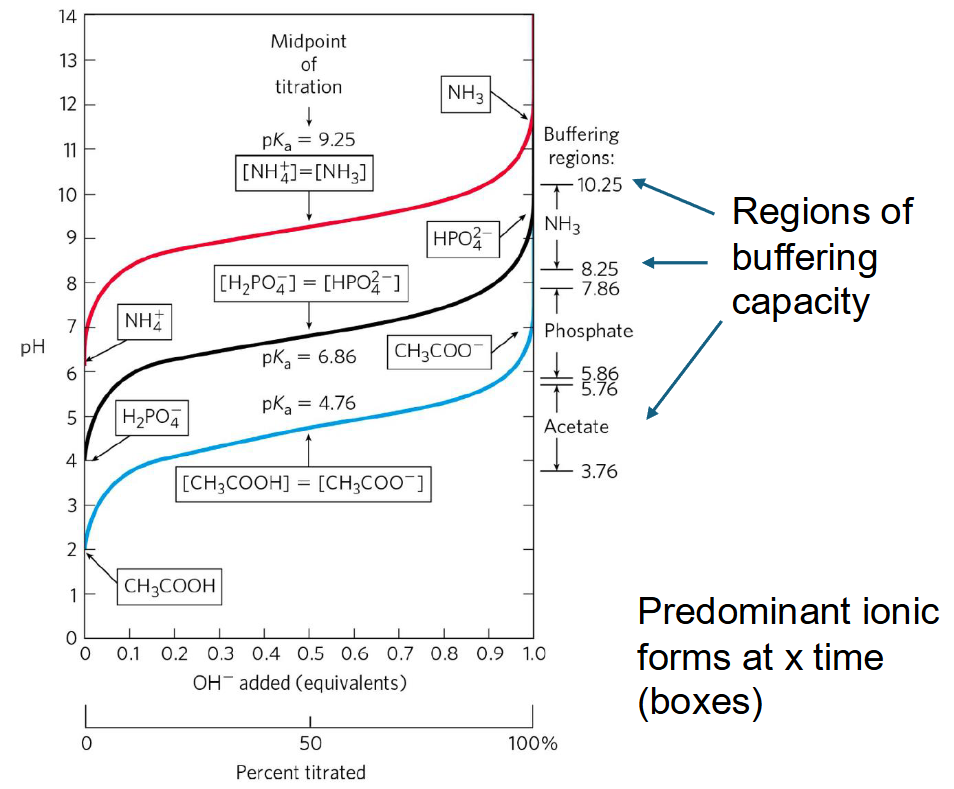
\includegraphics[scale=0.5]{L1_2.png}
\end{center}
\subsection*{Buffers are Mixtures of Weak Acids and Their Conjugate Bases}
\begin{itemize}
    \item buffers = aqueous systems that tend to resist changes in pH when small amounts of acid (\proton) or base (\hydroxide) are added
    \item a buffer system consists of a weak acid (the proton donor) and its conjugate acid (the proton acceptor)
    \item The \textbf{buffering region} is the flat zone of a titration curve (see above)
    \begin{itemize}
        \item the boundaries of a buffer system are pH = p\ka $\pm 1$ (so acetic acid buffer range is 3.76-5.76)
    \end{itemize}
\end{itemize}
\fbox{
    \parbox{\textwidth}{
        The buffering capacity is strongest when the ration of [HA] to [A$^-$] is close to 1:1.  This occurs at the p\ka of the weak acid, where half of the weak acid is dissociated.\\\\
        \textbf{If the ratio of acid to base (or base to acid) becomes too large -} greater than 10:1 or less than 1:10 - the buffer's capacity to neutralize added acids or bases weakens significantly
    }
}
\subsection*{The Henderson-Hasselbalch Equation Relates pH, p\ka, and Buffer Concentration}
\begin{itemize}
    \item \textbf{Henderson-Hasselbalch equation} = describes the shape of the titration curve of any weak acid
    \[\text{pH} = p\ka + \log \frac{[\text{A}^-]}{\text{HA}}\]
    \item Equation only works within the buffer region, outside of this it starts becoming inaccurate
\end{itemize}
\subsubsection*{Primary Uses of the Henderson-Hasselbalch Equation}
\begin{enumerate}
    \item Calculating pH of Buffers
    \begin{itemize}
        \item Predicts pH based on acid/base ratios
    \end{itemize}
    \item Designing Buffers
    \begin{itemize}
        \item Helps create buffers with a desired pH by adjusting the acid-base ratio.
    \end{itemize}
    \item Estimating p\ka
    \begin{itemize}
        \item Can determine the pKa of weak acids and bases experimentally
    \end{itemize}
\end{enumerate}
\subsection*{Deriving the Henderson-Hasselbalch Equation (not needed for exam)}
\begin{align*}
    K_a &= \frac{[\proton][\text{A}^-]}{[\text{HA}]}\\
    [\proton] &= K_a \cdot \frac{[\text{HA}]}{[\text{A}^-]}\\
    -\log [\proton] &= -\log K_a -\log \frac{[\text{HA}]}{[\text{A}^-]}\\
    \text{pH} &= \text{p\ka} -\log \frac{[\text{HA}]}{[\text{A}^-]}\\
    \text{pH} &= \text{p\ka} +\log \frac{[\text{A}^-]}{[\text{HA}]}
\end{align*}
\section*{Amino Acids}
\begin{itemize}
    \item In every living organism, proteins are constructed from a common set of 20 amino acids*
    \item Each amino acid has a side chain with distinctive chemical properties.  Amino acids may be regarded as the alphabet in which the language of protein structure is written.
\end{itemize}
\begin{center}
    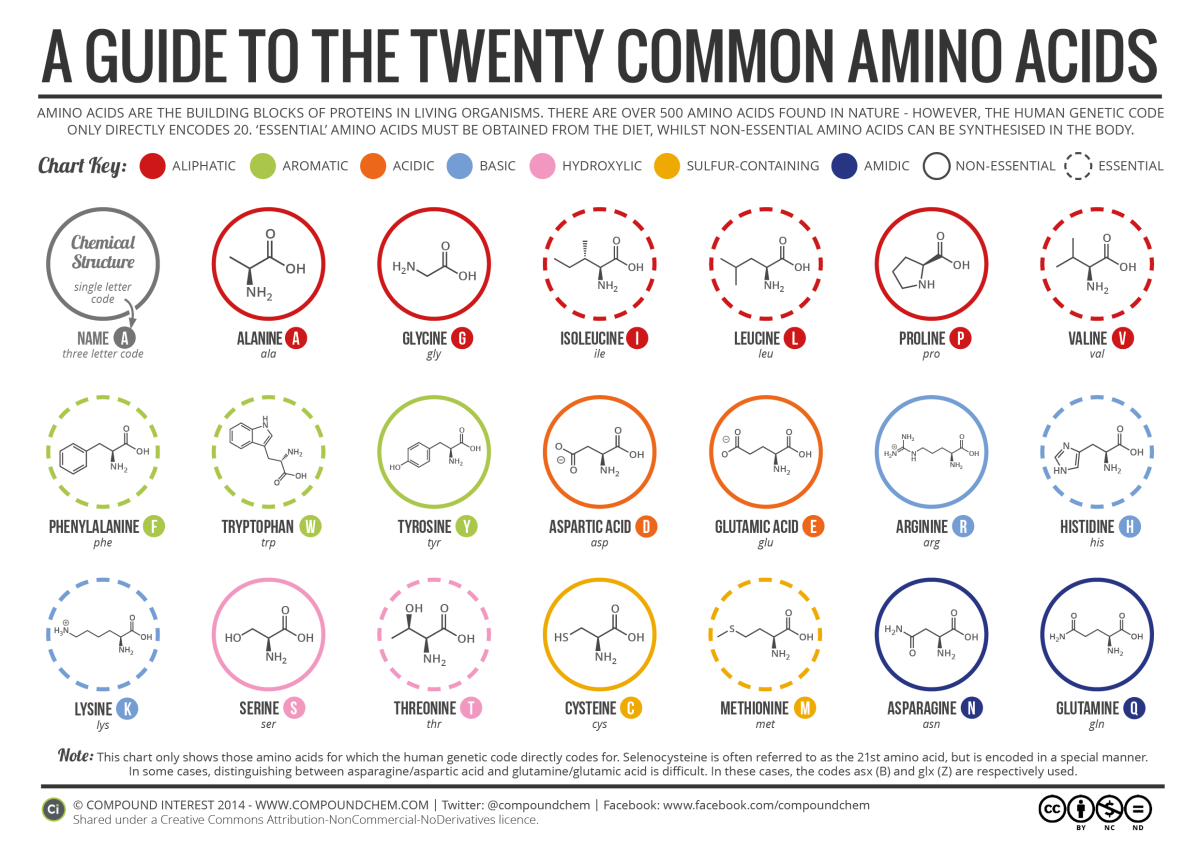
\includegraphics[width=\textwidth]{L1_4.png}
\end{center}
\subsection*{Amino Acids Share Common Structural Features}
\begin{itemize}
    \item $\alpha$ carbon and four substituents
    \item $\alpha$ carbon is the \textbf{chiral center} (except in Glycine, which is not chiral)
    \item Tetrahedral
\end{itemize}
The four substituents are:
\begin{itemize}
    \item a carboxyl group
    \item an amino group
    \item a hydrogen atom
    \item an \textbf{R group} (a side chain unique to each amino acid)
    \begin{itemize}
        \item \textbf{Glycine} has a second hydrogen atom instead of an R group.
    \end{itemize}
\end{itemize}   
\begin{center}
    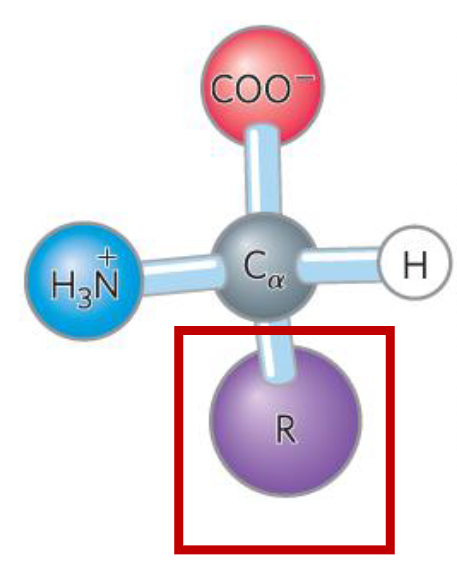
\includegraphics[scale=0.5]{L1_5.png}
\end{center}
\subsection*{The Amino Acid Residues in Proteins are L Stereoisomers}
\begin{itemize}
    \item Two possible stereoisomers = \textbf{enantiomers}
    \item \textbf{optically active} = polarize light is rotated in different directions by enantiomers (Glycine is the exception)
    \item D, L system specifies \textbf{absolute configuration}
\end{itemize}
\begin{center}
    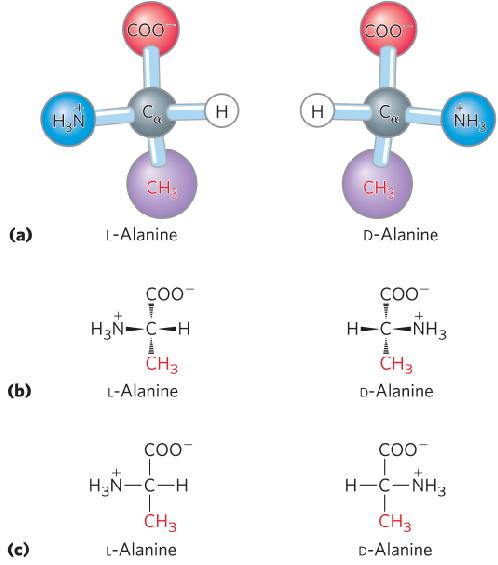
\includegraphics[scale=0.75]{L1_6.png}
\end{center}
\subsection*{Amino Acids can be classified by the R Group}
There are five main classes:
\begin{itemize}
    \item Nonpolar, aliphatic (7)
    \item Aromatic (3)
    \item Polar, uncharged (5)
    \item Positively charged, Basic (3)
    \item Negatively charged, Acidic (2)
\end{itemize}
\subsubsection*{Nonpolar, Aliphatic R Groups}
The \textbf{hydrophobic effect} stabilizes protein structure
\begin{itemize}
    \item Glycine
    \item Alanine
    \item Proline
    \item Valine
    \item Leucine
    \item Isoleucine
    \item Methionine
\end{itemize}

\subsubsection*{Aromatic R Groups}
R groups absorb UV light at 270-280 nm, and can contribute to the hydrophobic effect.
\begin{itemize}
    \item Phenylalanine
    \item Tyrosine
    \item Tryptophan
\end{itemize}

\subsubsection*{Polar, Uncharged R Groups}
R groups can \textbf{form hydrogen bonds}, and Cysteine can \textbf{form disulfide bonds}
\begin{itemize}
    \item Serine
    \item Threonine
    \item Cysteine
    \item Asparagine
    \item Glutamine
\end{itemize}

\subsubsection*{Positively Charged R Groups}
Have significant positive charge at pH 7.0.
\begin{itemize}
    \item Lysine
    \item Arginine
    \item Histidine
\end{itemize}

\subsubsection*{Negatively Charged R Groups}
Have net negative charge at pH 7.0.
\begin{itemize}
    \item Aspartate
    \item Glutamate
\end{itemize}
\subsection*{Essential Amino Acids}
\begin{center}
    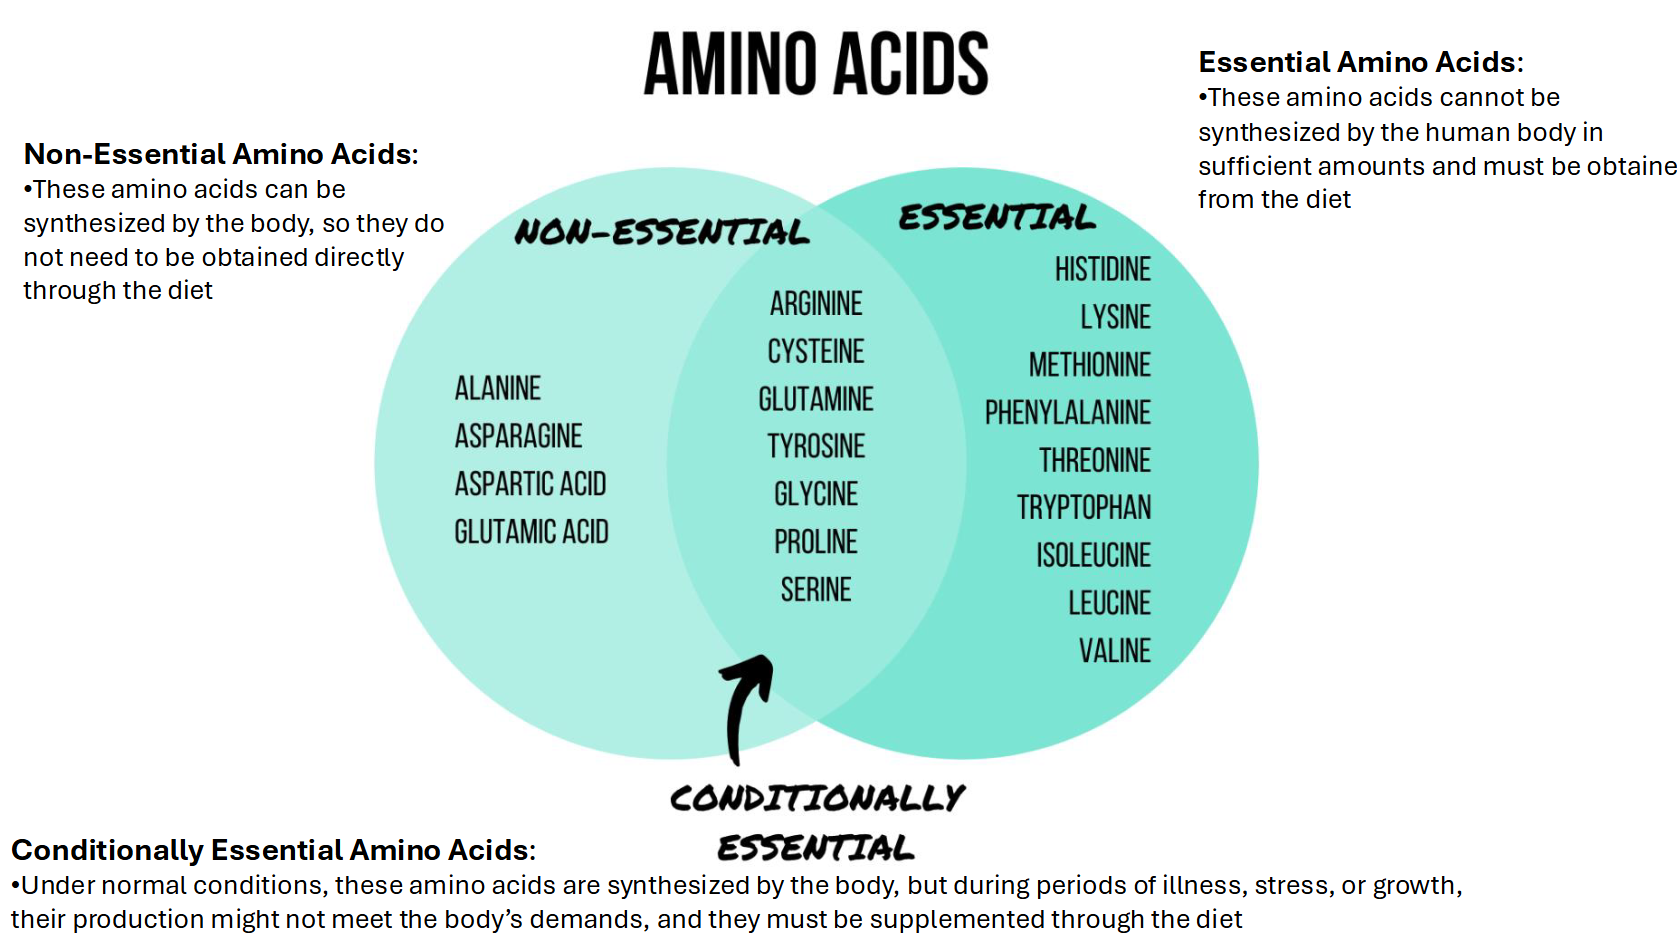
\includegraphics[width=\textwidth]{L1_7.png}
\end{center}
\subsection*{Amino Acids can act as Acids or Bases}
\begin{itemize}
    \item Amino acids are \textbf{acids}.  They are also \textbf{bases} containing an amino group.
    \item The term \textbf{amphoteric} is often used to describe amino acids, meaning that they are capable of acting as both acids and bases
    \item \textbf{zwitterion} occurs at neutral pH.
\end{itemize}
\begin{center}
    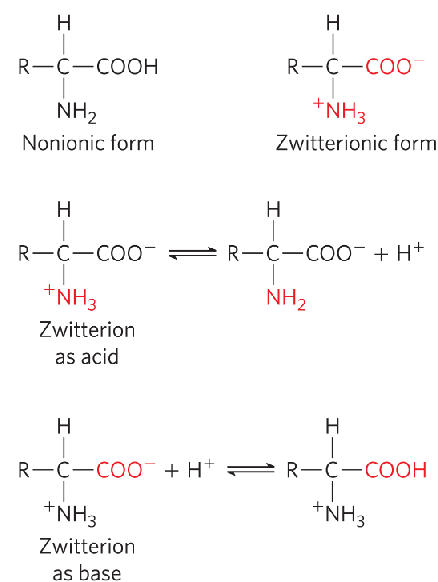
\includegraphics[scale=0.6]{L1_8.png}
\end{center}
\subsubsection*{The pH-dependent structures of a typical amino acid}
For a typical amino acid with a neutral sidechain \textbf{R}:
\begin{itemize}
    \item the positively charged form (+1) dominates at low pH.
    \item the zwitterionic (neutral) form dominates at intermediate pH, and
    \item the negatively charged form (-1) dominates at high pH.
\end{itemize}
\begin{center}
    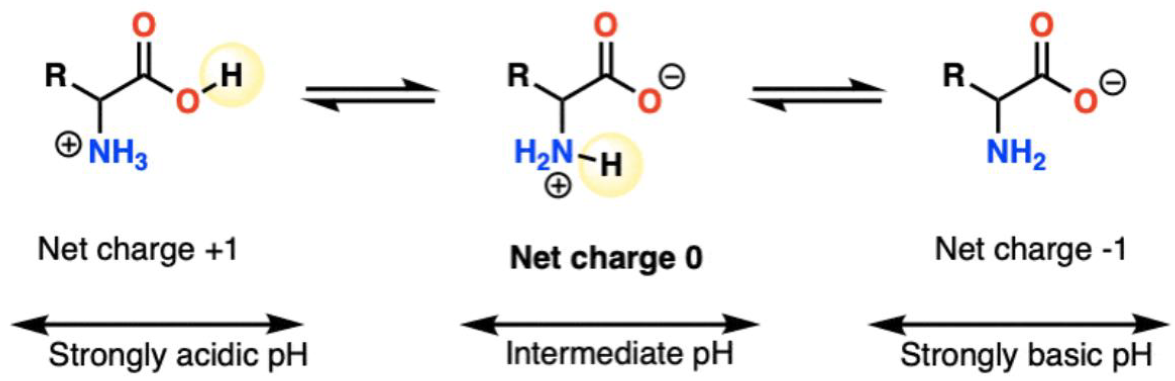
\includegraphics[width=\textwidth]{L1_9.png}
\end{center}
\subsection*{Effect of the Chemical Environment on p\ka}
\begin{itemize}
    \item $\alpha$-carboxyl group is more acidic than in carboxylic acids
    \item $\alpha$-amino group is less basic than in amines
\end{itemize}
\begin{center}
    \includegraphics*[width=\textwidth]{L1_10.png}
\end{center}
\subsection*{Structures (and p\ka) values of selected amino acids}
\begin{center}
    \includegraphics*[width=\textwidth]{L1_11.png}
\end{center}
\subsection*{Table of Amino Acid p\ka s}
\begin{center}
    \begin{tabular}{|lp{1cm}c|}
        \hline
        \textbf{Functional Group} &  & \textbf{p\ka} \\ \hline
        COO$^-$ -terminus &  & 3.5 \\ \hline
        $^+$NH$_3$-terminus &  & 8.5 \\ \hline
        $\alpha$-COO$^-$ (free amino acid) &  & 2 \\ \hline
        $\alpha$-$^+$NH$_3$ (free amino acid) &  & 9.5 \\ \hline
        Aspartate R group &  & 3.9 \\ \hline
        Glutamate R group &  & 4.3 \\ \hline
        Histidine R group &  & 6 \\ \hline
        Cysteine R group &  & 8.3 \\ \hline
        Tyrosine R group &  & 10 \\ \hline
        Lysine R group &  & 10.8 \\ \hline
        Arginine R group &  & 12.5 \\ \hline
        \end{tabular}
\end{center}
\section*{Titration of Amino Acids}
\begin{itemize}
    \item Cation $\rightleftharpoons$ zwitterion $\rightleftharpoons$ anion
    \item -COOH (carboxyl) has an acidic p\ka~(p$K_1$)
    \item -NH$_3^+$ (amino) has a basic p\ka~(p$K_2$)
    \item the pH at which the net electric charge is zero is the \textbf{isoelectric point (pI)}
\end{itemize}
\begin{center}
    \includegraphics*[scale=0.7]{L2_1.png}
\end{center}
This titration curve is a qualititative measure of the p\ka of each ionizing group.
\begin{itemize}
    \item shows buffering power 
    \begin{itemize}
        \item flat regions are buffer regions. Glycine has two, one centered at p$K_1 = 2.34$, the other at p$K_2 = 9.6$
        \item Buffer regions are highlighted in blue.
    \end{itemize}
    \item shows relationship between its net charge and the pH of the solution
    \begin{itemize}
        \item isoelectric point, or pI, can be calculated
    \end{itemize}
    \item In the above image, glycine is present predominantly as its dipolar form, fully ionized with no net electric charge.  At the point (pH = 5.97, 1eq base), glycine has an equal number of positive and negative charges.
\end{itemize}
\subsection*{The Isoelectric Point}
\begin{itemize}
    \item The \textbf{isoelectric point (pI)} determines the pH at which a molecule carries no net electric charge
    \item This occurs when the positive and negative charges on the molecule are balanced.  For amino acids, the pI is determined by the p$Ka$ values of its ionizable groups, such as the amino (-NH$_3^+$) and carboxyl (-COOH) groups, and sometimes the side chain, if it is ionizable.
    \item \underline{for amino acids without ionizable side chains}, the \textbf{isoelectric point (pI)} is:
    \[\text{pI} = \frac{\text{p}K_1 + \text{p}K_2}{2}\]
    \item pH = pI = net charge is zero (amino acid least soluble in water, does not migrate in electric field)
    \item pH > pI = net negative charge
    \item pH < pI = net positive charge
\end{itemize}
\subsection*{Isoelectric point - Alanine}
\begin{center}
    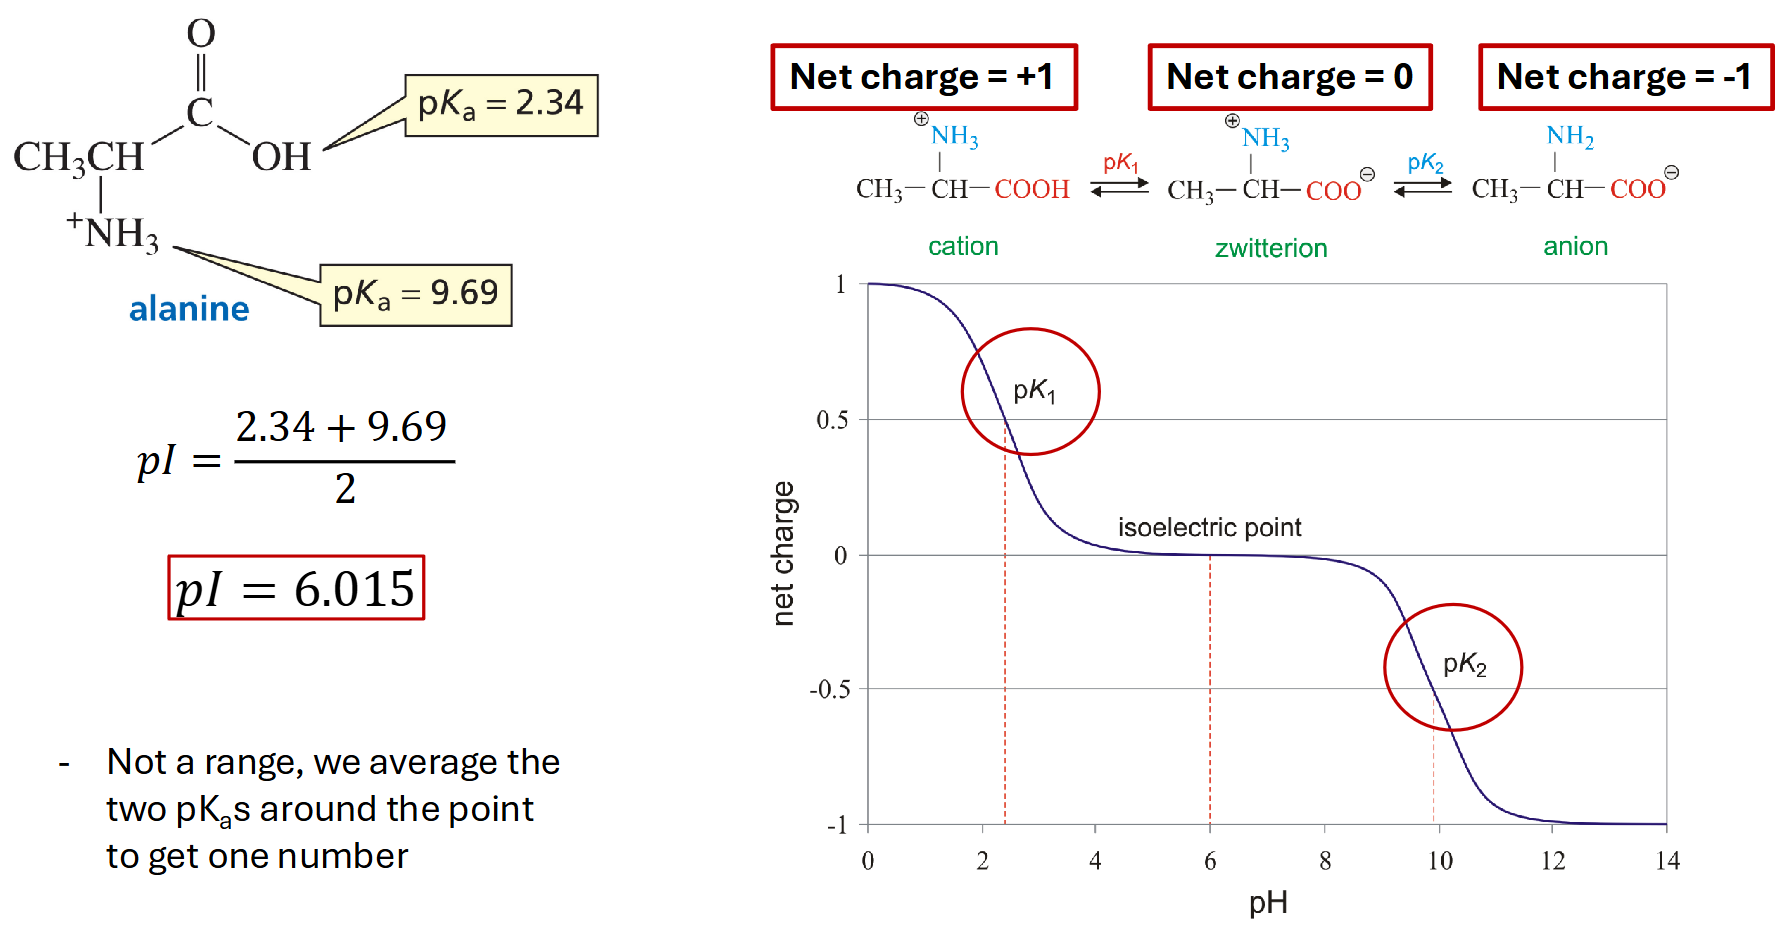
\includegraphics[width=\textwidth]{L2_2.png}
    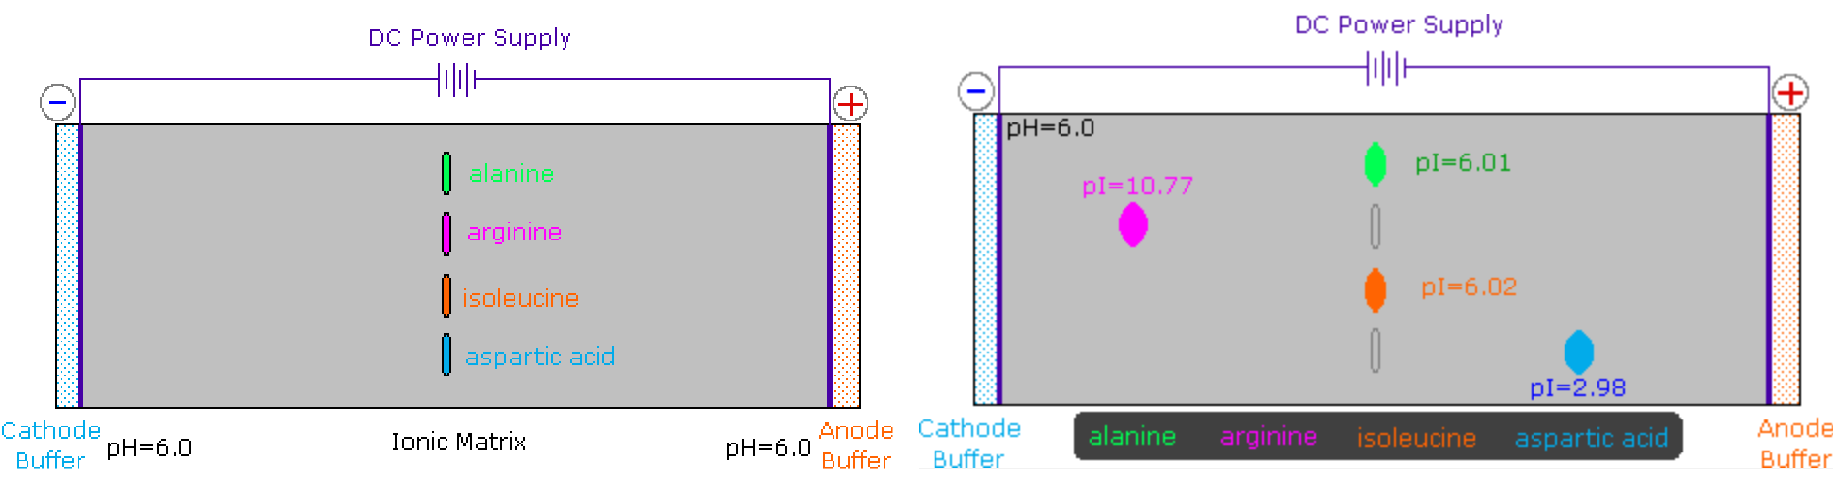
\includegraphics[width=\textwidth]{L2_3.png}
\end{center}
\subsection*{Tyrosine at different pH}
\subsubsection*{Standard Representation}
\begin{center}
\includegraphics*[scale=0.8]{L2_4.png}
\end{center}
\begin{itemize}
    \item This is the standard representation of Tyrosine, found in many online sources and textbooks
    \item It is important to note that \textbf{this structure does not exist at any pH}!
    \item The molecule is made neutral just because, to display its structure.
\end{itemize}
\subsubsection*{Representations at different pH}
\begin{center}
    \includegraphics*[width=\textwidth]{L2_5.png}
\end{center}
\subsubsection*{Titration of Tyrosine}
\begin{center}
    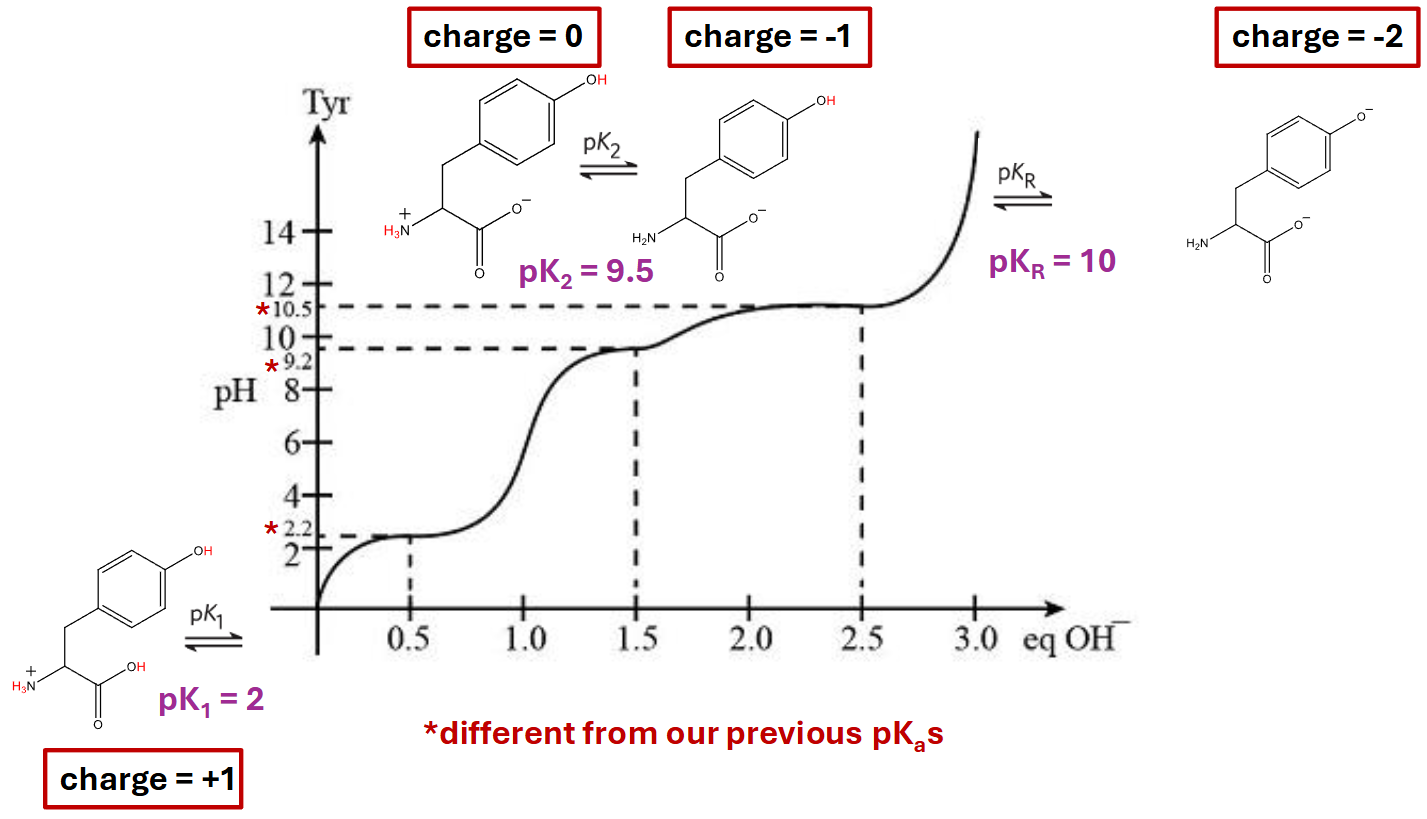
\includegraphics[width=\textwidth]{L2_6.png}
\end{center}
\begin{itemize}
    \item Notice there is a buffer region around each p\ka
\end{itemize}
\subsection*{Titration of Amino Acids with an Ionizable R Group}
\begin{center}
    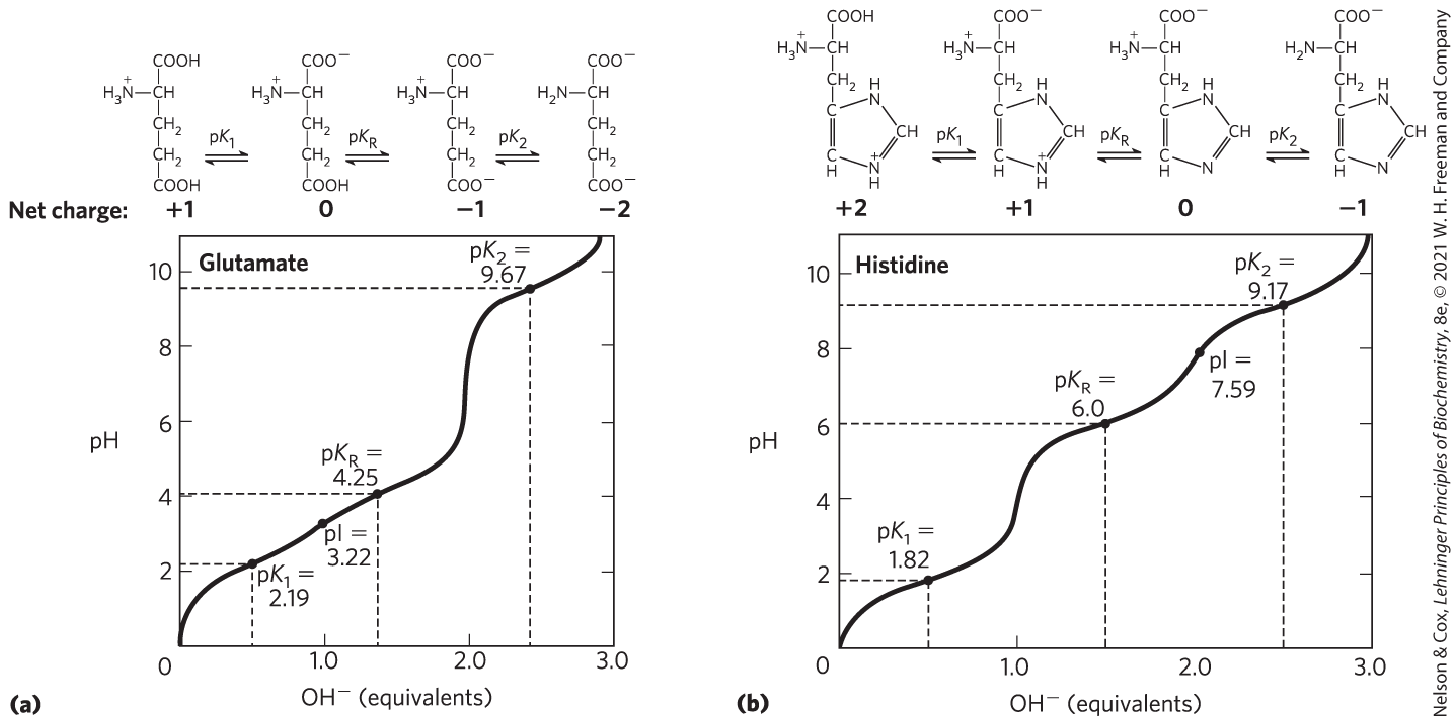
\includegraphics[width=\textwidth]{L2_7.png}
\end{center}
\section*{Peptides and Proteins}
\textbf{In proteins, amino acids are joined in characteristic linear sequences through a common amide linkage, the peptide bond.}  The amino acid sequence of a protein constitutes its primary structure.
\begin{itemize}
    \item Peptides are chains of amino acids
    \item Peptide bond:
    \begin{itemize}
        \item Covalent
        \item formed through \textbf{condensation}
        \item broken through \textbf{hydrolysis}
    \end{itemize}
    \item The \textbf{carboxyl group} of one amino acid loses a hydroxyl group (-OH)
    \item The \textbf{amino group} of the second amino acid loses a hydrogen atom (-H)
\end{itemize}
\begin{center}
    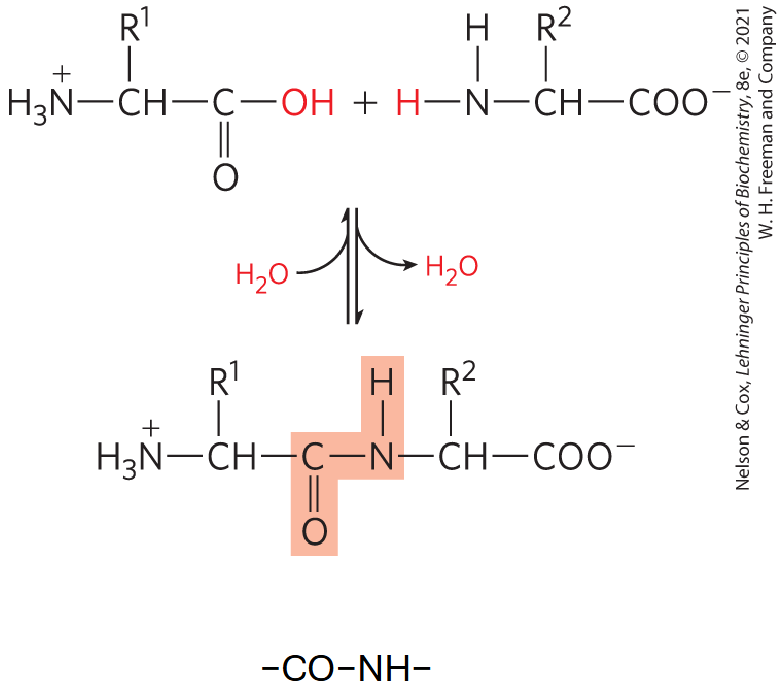
\includegraphics[width=\textwidth]{L2_9.png}
\end{center}
\subsection*{Peptide Types by the Number}
\begin{itemize}
    \item dipeptide = 2 amino acids, 1 peptide bond
    \item tripeptide = 3 amino acids, 2 peptide bonds
    \item \textbf{oligopeptide} = a few amino acids
    \item \textbf{polypeptide} = many amino acids, molecular weight < 10 kDa
    \item \textbf{protein} = thousands of amino acids, molecular weight > 10 kDa
\end{itemize}
\subsubsection*{Aside: Daltons}
\begin{itemize}
    \item The average molecular weight of an amino acid is 110Da.
    \item Dalton (Da) is an alternate name for the atomic mass unit, and kilodalton (kDa) is 1000 daltons
    \item Thus, a protein with a mass of 64kDa has a molecular weight of 64,000 grams per mole
\end{itemize}
\subsection*{Peptide Terminals}
Convention: numbering (and naming) starts from the \textbf{amino-terminal residue} ($N$-terminal)
\begin{center}
    \includegraphics*[width=\textwidth]{L2_10.png}
\end{center}
\subsection*{Naming Peptides}
\begin{itemize}
    \item Full amino acid names: serylglycyltyrosylalanylleucine
    \item Three letter code abbreviations: Ser-Gly-Tyr-Ala-Leu
    \item One letter code abbreviation: SGYAL
\end{itemize}
\subsection*{Peptides can be distinguished by their ionization behavior}
\begin{itemize}
    \item Ionizable groups in peptides:
    \begin{itemize}
        \item one free $\alpha$-amino group
        \item one free $\alpha$-carboxyl group
        \item some R groups
    \end{itemize}
\end{itemize}
\begin{center}
    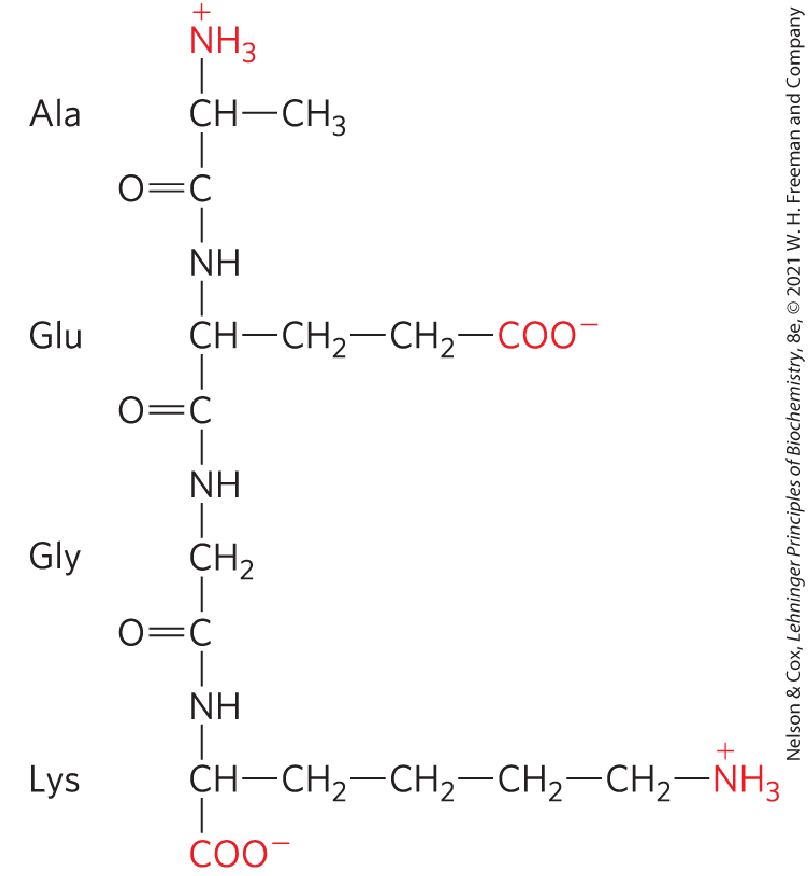
\includegraphics[scale=0.7]{L2_11.png}
\end{center}
\subsection*{Drawing oligopeptides}
\textbf{Draw the oligopeptide Gly-Asp-Tyr-Arg at physiological pH}
\begin{center}
    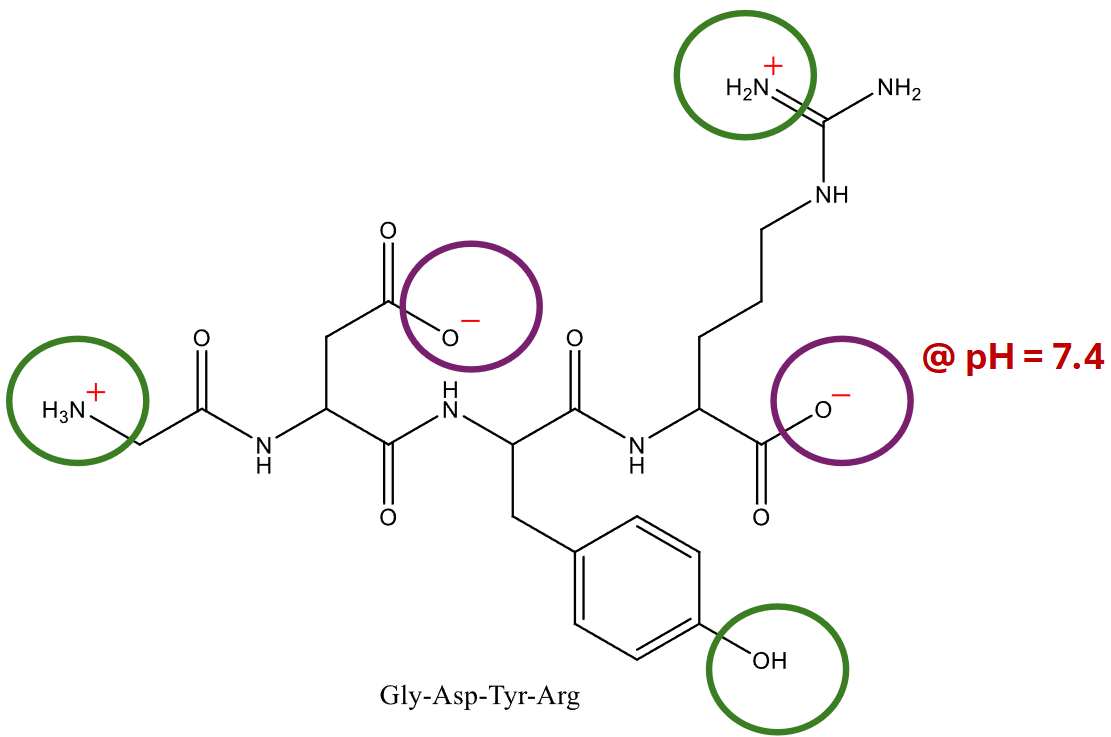
\includegraphics[width=\textwidth]{L2_12.png}
\end{center}
\begin{itemize}
    \item Refer to the functional group pH table earlier in this document.
    \item pH < pKa: The molecule is protonated (it holds onto its protons)
    \item pH > pKa: The molecule is deprotonated (it loses its protons)
\end{itemize}
\subsection*{Determining pI of peptide}
\begin{enumerate}
    \item Draw the peptide at its most protonated form (low pH)
    \item Calculate overall charge
    \item Calculate the change in charge as pH rises (noting p\ka s)
    \item Use the 2 p\ka s surrounding peptide at 0 charge $\rightarrow$ average
\end{enumerate}
\begin{center}
    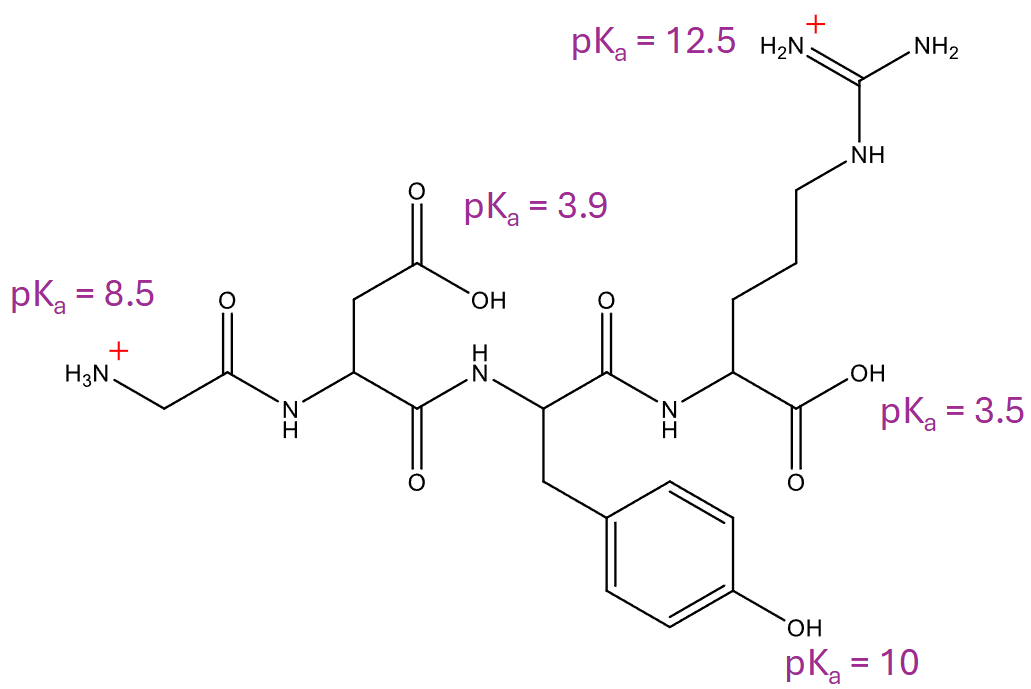
\includegraphics[width=\textwidth]{L2_13.png}
    \begin{tabular}{|c|c|c|c|c|c|c|}
        \hline
        \textbf{pH range} & \textless 3.5 & 3.5 - 3.9 & 3.9 - 8.5 & 8.5 - 10 & 10 - 12.5 & \textgreater 12.5 \\ \hline
        \textbf{$\sim$net charge} & +2 & +1 & 0 & -1 & -2 & -3 \\ \hline
    \end{tabular}
\end{center}
\[\text{pI} = \frac{8.5 + 3.9}{2} \boxed{= 6.2}\]
\section*{Intermolecular Interactions within Proteins}
\subsection*{Ionic Bonds}
\begin{itemize}
    \item Strong electrostatic forces of attraction between oppositely charged ions
    \item Protein structures are formed by the interactions of amino acid side chains
    \item If an acidic chain and a basic side chain interact (e.g., Glu and Lys) \textbf{both an ionic interaction and a hydrogen bond will form}
    \item This is called a \textbf{salt bridge} - but most of the strength of this interaction comes from the opposing charges
\end{itemize}
\begin{center}
    \includegraphics*[scale=0.6]{L3_1.png}
\end{center}

\subsection*{Induced Dipoles - London Dispersion Forces (LDFs)}
\begin{itemize}
    \item The weakest intermolecular force
    \item The LDF is a temporary attractive force that results when \textbf{the electrons in two adjacent atoms occupy positions that make the atoms form temporary dipoles.}  This force is sometimes called an induced dipole-induced dipole attraction.
    \item This is (often) the predominant force between nonpolar molecules
    \item The London dispersion force is sometimes called a 'Van der Waals force.'  Van der Waals force is a general term that describes any attractive intermolecular force between molecules and includes both the London dispersion force and the dipole-dipole force
\end{itemize}
\begin{center}
    \includegraphics*[width=\textwidth]{L3_2.png}
\end{center}
\subsection*{Micelle - Where are the LDFs?}
LDFs are primarily found among the hydrophobic (nonpolar) tails of the amphiphilic molecules (like fatty acids or detergents) that form the core of the micelle.
\begin{center}
    \includegraphics*[width=\textwidth]{L3_3.png}
\end{center}
LDFs contribute to the stability of the micelle by keeping the nonpolar tails in close proximity in the micelle's core

\subsection*{Dipole-dipole interactions}
Attractive forces that occur between polar molecules, where permanent dipoles are present due to the uneven distribution of electrons
\begin{itemize}
    \item Dipole-dipole interactions are generally stronger than London dispersion forces but weaker than hydrogen bonds or ionic interactions.
\end{itemize}
\begin{center}
    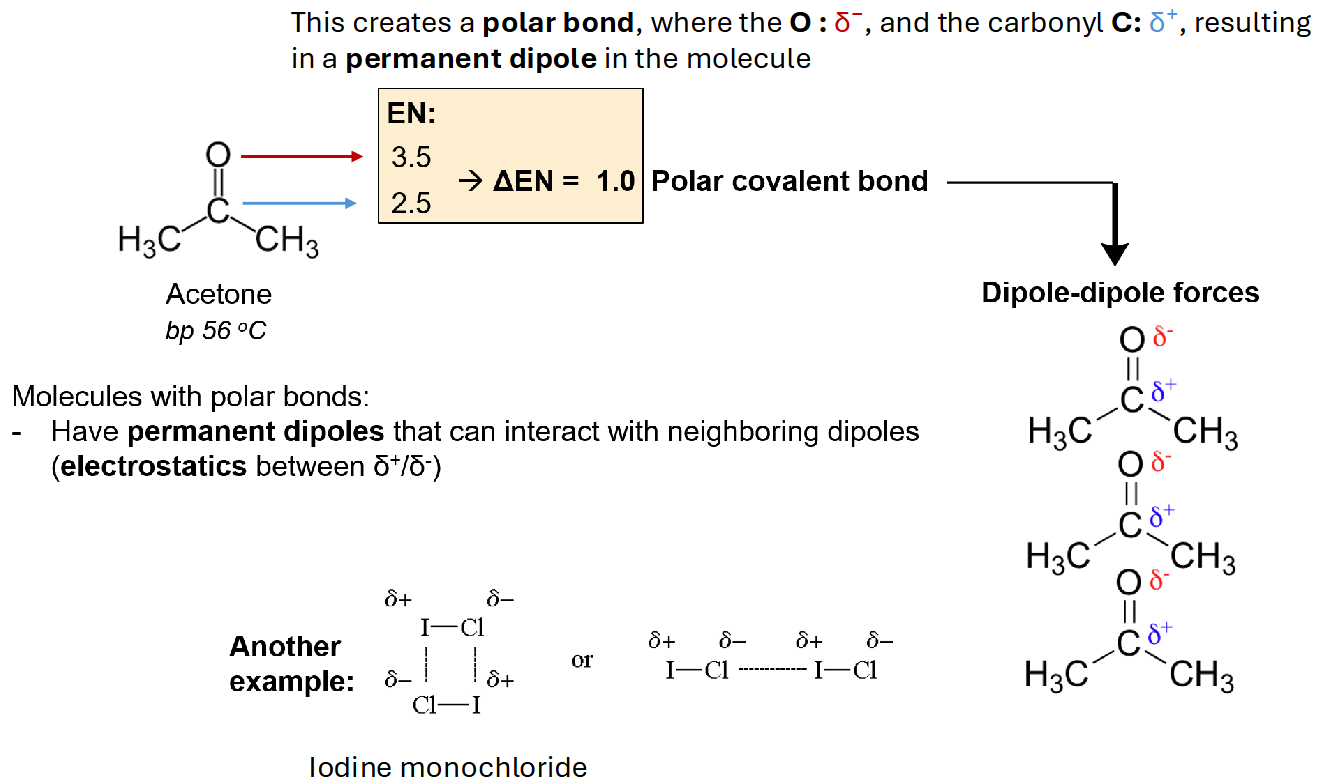
\includegraphics[width=\textwidth]{L3_4.png}
\end{center}

\subsection*{$\pi$-stacking interactions}
\begin{itemize}
    \item Non-covalent interactions that occur between aromatic rings, where the delocalized $\pi$-electrons in thes systems interact with each other.
    \item Cyclic aromatic compounds have $\pi$ orbital rings stacked above and below the molecular structure.
\end{itemize}
\begin{center}
    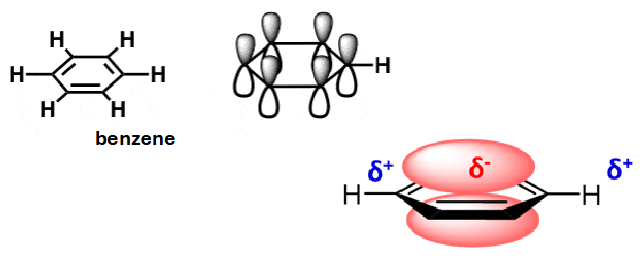
\includegraphics[scale=0.8]{L3_5.png}
    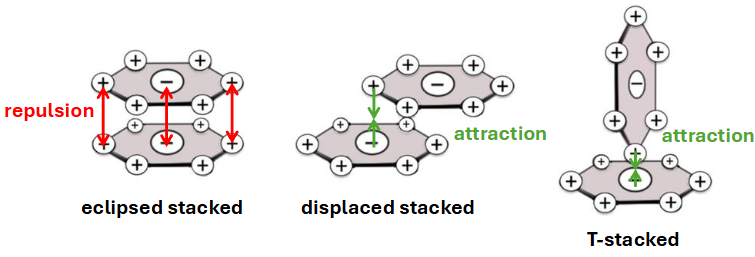
\includegraphics[width=\textwidth]{L3_6.png}
    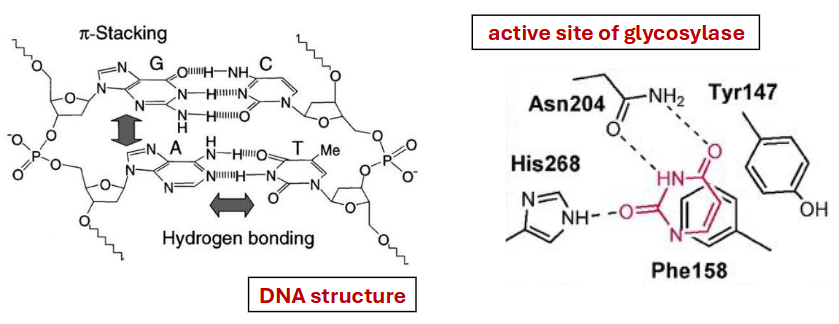
\includegraphics[width=\textwidth]{L3_7.png}
\end{center}

\subsection*{Importance of Non-Covalent Interactions}
\begin{enumerate}
    \item Protein Folding and Stability: Hydrogen bonds, hydrophobic interactions, ionic interactions, and van der Waals forces contribute to the folding of proteins into their three- dimensional structures. These forces also help stabilize protein structures, such as maintaining the secondary, tertiary, and quaternary structures
    \item DNA Double Helix: Hydrogen bonds between complementary bases (A-T and G-C) and $\pi$-$\pi$ stacking interactions between the aromatic bases help stabilize the DNA double helix structure
    \item Membrane Formation: Hydrophobic interactions between the fatty acid tails of phospholipids drive the formation of lipid bilayers, which form the basic structure of cell membranes
    \item Enzyme-Substrate Binding: Play a key role in the binding of enzymes to their substrates or cofactors, allowing for specificity and reversibility in catalysis
    \item Molecular Recognition: Participate in the recognition of molecules such as ligands by receptors, or antigens by antibodies, facilitating many biological processes such as signal transduction and immune responses
\end{enumerate}

\section*{The Thermodynamic Problem}
\begin{itemize}
    \item Living cells must constantly perform work, such as building complex molecules, transporting substances, and maintaining ion gradients, to stay alive. This requires an understanding of \textbf{thermodynamic principles} to predict which processes can occur naturally and how energy flows in biological systems
\end{itemize}
\subsection*{First Law of Thermodynamics}
\textbf{Energy Conservation: Energy cannot be created or destroyed, only transformed}
\begin{itemize}
    \item $\Delta$G tells us how much energy is available to do work
    \item $\Delta$H (enthalpy) represents the heat exchanged in a system
    \item Example: In cellular respiration, glucose releases energy ($\Delta$H < 0) that is used to produce ATP. Energy is transformed but conserved
\end{itemize}

\subsection*{Second Law of Thermodynamics}
\textbf{Entropy of the universe always increases in spontaneous processes}
\begin{itemize}
    \item $\Delta$S (entropy) is a measure of disorder
    \item $\Delta G = \Delta H - T\Delta S$: A negative $\Delta$G means a process is spontaneous and aligns with the second law (entropy increases)
    \item Even if a system's entropy decreases ($\Delta$S < 0), the surroundings must increase entropy for the reaction to be spontaneous
    \item Example: Protein folding is spontaneous ($\Delta$G < 0) even though it decreases system entropy, because heat is released, increasing the entropy of the surroundings
\end{itemize}

\subsection*{Third Law of Thermodynamics}
\textbf{As temperature approaches absolute zero, entropy approaches zero}
\begin{itemize}
    \item At very low temperatures, T$\Delta$S becomes small, and $\Delta$H dominates
    \item Spontaneous processes at low temperatures: Exothermic reactions ($\Delta$H < 0) are more likely to be spontaneous when entropy is low
    \item Example: Water freezing is spontaneous at low temperatures because it releases heat ($\Delta$H < 0) even though it decreases disorder ($\Delta$S < 0)
\end{itemize}

\subsection*{Gibbs Free Energy (G)}
\begin{itemize}
    \item \textbf{Gibbs free energy (G)} represents the maximum amount of energy available to perform work in a system. It's the key to understanding how cells manage energy.
    \item The \textbf{Gibbs free energy change ($\Delta$G)} tells us the difference in available free energy between reactants and products. It determines whether a process will occur spontaneously (i.e., without needing an external energy input).
    \item $\Delta$G determines the spontaneity of a process
\end{itemize}

\subsection*{Reaction Coordinate Diagram}
\begin{itemize}
    \item A reaction coordinate diagram shows the progress of a reaction vs the overall free energy (G) as it proceeds
    \begin{itemize}
        \item Energy flowing downhill is favorable, uphill is unfavorable.
    \end{itemize}
\end{itemize}
\begin{center}
    \includegraphics*[scale=0.6]{L3_8.png}
\end{center}

\subsection*{Spontaneity and $\Delta$G: What it Really Means}
\begin{itemize}
    \item \textbf{If $\Delta$G > 0, the process is non-spontaneous} (it requires an input of energy to occur).  This type of reaction is called \textbf{endergonic}.
    \begin{itemize}
        \item \textbf{Example:} The synthesis of \textbf{glucose} from CO$_2$ and water during \textbf{photosynthesis} is endergonic ($\Delta$G > 0).  Plants need energy from sunlight to drive this process because it doesn't happen spontaneously
    \end{itemize}
    \item \textbf{Why:} It makes sense - if the $\Delta$G is positive, how could you get more work out of a system without putting energy into it?  In biological systems, cells \textbf{couple} endergonic reactions with exergonic ones to make them proceed.
\end{itemize}
\begin{center}
    \includegraphics*[scale=0.9]{L3_9.png}
\end{center}
\begin{itemize}
    \item \textbf{If $\Delta$G < 0, the process is spontaneous} (it can occur naturally without additional energy input).  This is called an \textbf{exergonic} process.
    \begin{itemize}
        \item \textbf{Example:} The breakdown of \textbf{glucose} during \textbf{cellular respiration} is exergonic ($\Delta$G < 0).  When glucose is metabolized into CO$_2$ and \water, energy is released that cells can use to drive other processes (like making ATP).
    \end{itemize}
    \item \textbf{Why:} Energy is released when bonds in glucose are broken, allowing the system to do work - such as moving ions, powering cellular machinery, or synthesizing molecules.  The process moves towards equilibrium, where the system is most stable.
\end{itemize}
\begin{center}
    \includegraphics*[scale=0.9]{L3_10.png}
\end{center}
\subsubsection*{However}
\begin{itemize}
    \item In \textbf{biological systems, true equilibrium} is rarely reached because cells operate under a \textbf{steady state} rather than equilibrium
    \item In a steady state, the concentrations of molecules like glucose and ATP are kept constant, but continuous input of reactants (like glucose) and removal of products (like CO$_2$) allow work to be performed
    \item If equilibrium were reached, the system would be in a \textbf{low-energy state}, and no further work could be done. This is why biological systems keep reactions away from equilibrium to continue performing work
\end{itemize}
\begin{itemize}
    \item \textbf{If $\Delta$G = 0, the system is at equilibrium}, meaning there's no net change in the reactants or products, and no work can be done.  This happens when the forward and reverse reactions occur at the same rate.
    \begin{itemize}
        \item \textbf{Example:} Consider \textbf{ATP} in equilibrium with \textbf{ADP} and inorganic phosphate (P$_\text{i}$) in a cell.  If the reaction reaches equilibrium, no energy would be released or consumed, making it impossible for the cell to do any work involving ATP.
    \end{itemize}
\end{itemize}
\begin{center}
    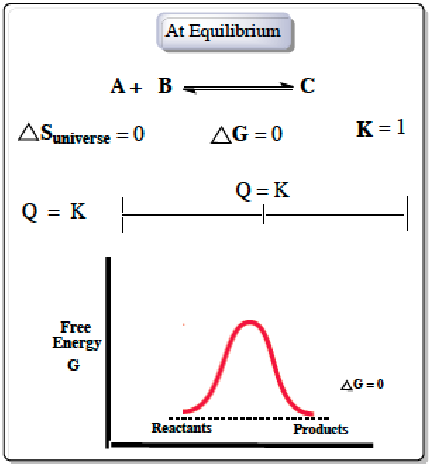
\includegraphics[scale=0.9]{L3_11.png}
\end{center}

\subsection*{How Cells Use $\Delta$G to Perform Work: Reaction Coupling}
\begin{itemize}
    \item Cells often use \textbf{reaction coupling} to make non-spontaneous processes occur.  By coupling a reaction with \textbf{positive $\Delta$G} (endergonic) to one with \textbf{negative $\Delta$G} (exergonic), the overall process can still be spontaneous
    \begin{itemize}
        \item \textbf{Example:} The phosphorylation of glucose in the first step of \textbf{glycolysis} ($\Delta$G > 0) is coupled with the \textbf{hydrolysis of ATP} to ADP and P$_\text{i}$ ($\Delta$G < 0).  \textbf{Together, these reactions allow glucose to be phosphorylated and the overall process to move forward with a net negative $\Delta$G}
        \item \textbf{Key Insight:} Cells use ATP as sort of "energy currency" to drive many otherwise non-spontaneous reactions.  ATP hydrolysis ($\Delta$G < 0) provides the energy necessary to make those reactions happen
    \end{itemize}
\end{itemize}

\subsection*{Coupled Reactions}
\begin{itemize}
    \item How does biochemistry pull off an anabolic reaction?
    \begin{itemize}
        \item By coupling it with an energetically favorable reaction (the classic example is the hydrolysis of ATP)
        \item i.e., coupling an endergonic reaction with an exergonic reaction
    \end{itemize}
\end{itemize}
\begin{center}
    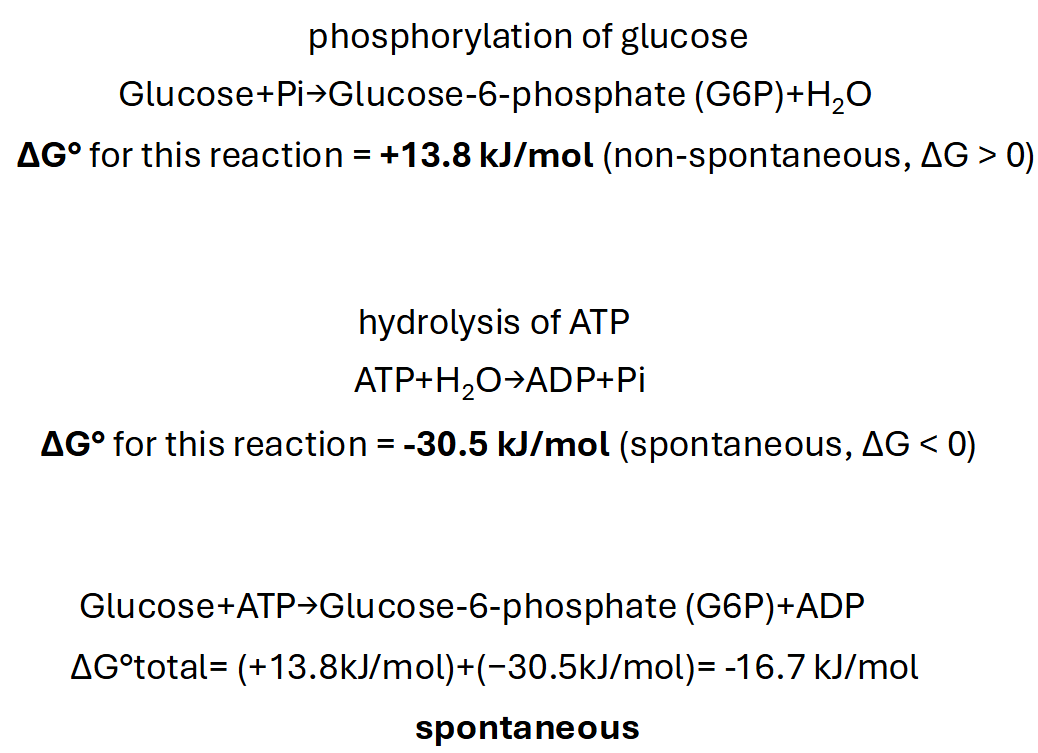
\includegraphics[width=\textwidth]{L3_12.png}
\end{center}

\subsection*{Quantifying $\Delta$G - Enthalpy}
\[\Delta G^\circ = \Delta H^\circ - T\Delta S^\circ\]
\begin{itemize}
    \item H, enthalpy is the heat content locked in a system
    \item $\Delta$H is the change in enthalpy
\end{itemize}
Equivalent to the difference between bonds/interactions formed and bonds/interactions broken
\begin{itemize}
    \item \textbf{Bond formation} typically \textbf{releases energy} because when atoms form bonds, they move to a lower energy state.  This means that energy is released as the atoms become more stable
    \item \textbf{Bond breaking} generally \textbf{requires energy input} because energy must be provided to overcome the stability of the bond and separate the atoms, moving them to a higher energy state
\end{itemize}

\subsection*{Quantifying $\Delta$G - Entropy}
\begin{itemize}
    \item S, entropy is the degree of disorder in a system
    \item $\Delta$S is the change in entropy
\end{itemize}
Equivalent to disorder of products minus disorder of reactants
\begin{itemize}
    \item \textbf{Systems tend toward disorder}
\end{itemize}
\begin{center}
    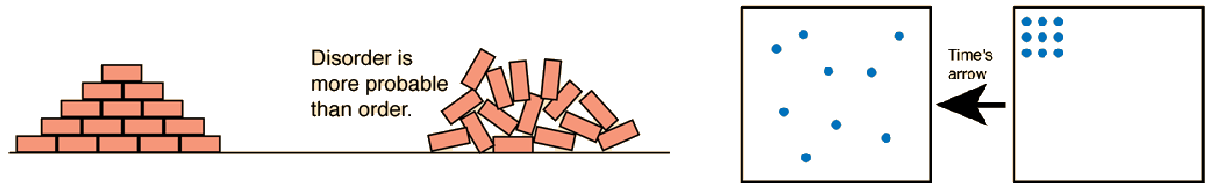
\includegraphics[width=\textwidth]{L3_13.png}
\end{center}
\end{document}
